% 1977 年福建卷理科第 5 题：障碍物两侧测距示意图
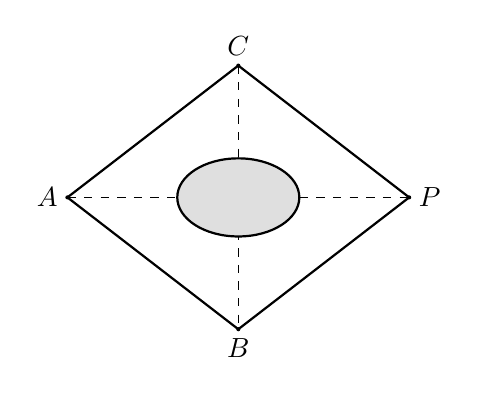
\begin{tikzpicture}[scale=0.62]
  \coordinate (A) at (0,0);
  \coordinate (P) at (7.0,0);
  \coordinate (C) at (3.5,2.7);
  \coordinate (B) at (3.5,-2.7);
  \draw[thick] (A)--(C)--(P)--(B)--cycle;
  \draw[dashed] (A)--(P);
  \draw[dashed] (C)--(B);
  \fill[gray!25] (3.5,0) ellipse (1.25 and 0.8);
  \draw[thick] (3.5,0) ellipse (1.25 and 0.8);
  \fill (A) circle (1.2pt) node[left] {$A$};
  \fill (P) circle (1.2pt) node[right] {$P$};
  \fill (C) circle (1.2pt) node[above] {$C$};
  \fill (B) circle (1.2pt) node[below] {$B$};
\end{tikzpicture}
